%%=============================================================================
%% Methodologie
%%=============================================================================

\chapter{\IfLanguageName{dutch}{Methodologie}{Methodology}}%
\label{ch:methodologie}

%% TODO: Hoe ben je te werk gegaan? Verdeel je onderzoek in grote fasen, en
%% licht in elke fase toe welke stappen je gevolgd hebt. Verantwoord waarom je
%% op deze manier te werk gegaan bent. Je moet kunnen aantonen dat je de best
%% mogelijke manier toegepast hebt om een antwoord te vinden op de
%% onderzoeksvraag.
\section{Switch van aanpak}
Het oorspronkelijke plan was om een tool te schrijven die (deels) stappen bij het proces van een webshop overname kan versnellen. Rekening houdende met de werkwijze van Team Made mag deze tool niet te complex zijn, en moet naar toekomstig gebruik toe gemakkelijk schaalbaar zijn.
\\\\
Echter tijdens het schrijven van het voorstel voor deze bachelorproef waren AI-tools zoals ChatGPT nog onbestaand. Het is na de literatuurstudie heel erg duidelijk geworden dat met behulp van (een combinatie van) AI-tools Team Made zijn doel kan bereiken. De auteur heeft in de loop van het schrijven ondervonden dat veel programmeurs, waaronder hijzelf, dagelijks code laten genereren door ChatGPT. Deze chatbot is doorheen de loop van tijd ook meermaals van updates voorzien en aanzienlijk veel sneller geworden. 
\\\\
De hele opzet van WordPress is geautomatiseerd met behulp van scriptie in PowerShell. Het overnemen van bestaande webshops hun designs en data kan verwezenlijkt worden door een combinatie van manueel programmeerwerk en AI-tools te gebruiken. 
\section{Analyse}
De bestaande AI-tools (tijdens de periode van de literatuurstudie) worden aandachtig doorlopen en direct op de proef gesteld door (stukken van) een webshop van Team Made hun lijst na te maken als template. Deze templates moeten zo dicht mogelijk aanleunen bij het gewenste resultaat (de oorspronkelijke webshop). Vervolgens bekijken we of de AI-tools instaat zijn om data te voorzien op deze templates. Merk op dat veel (nieuwe) AI-tools op moment van schrijven nog in ontwikkeling zijn.
\label{ai_tools_programmeren}\subsection{AI-tools voor te programmeren}
Onderstaande AI-tools kunnen gebruikt worden om code uit te leggen en te laten genereren. Dit zijn handige hulpmiddelen om te programmeren met elk hun eigen voor- en nadelen. Op moment van schrijven heeft ChatGPT een 'Plus'\footnote{\href{https://openai.com/blog/chatgpt-plus}{https://openai.com/blog/chatgpt-plus}} optie die 20 dollar per maand kost. Hiermee is de tool meer beschikbaar (minder downtime van de server), worden de antwoorden sneller weergegeven en zijn nieuwe uitbreidingen sneller toegankelijk. Deze optie is niet uitgetest, maar kan interessant zijn als beschikbaarheid een belangrijke factor speelt. Zie figuur \ref{vergelijking_ai_tools_programmeren} voor een korte vergelijkende studie tussen deze AI-tools.  
\begin{itemize}
    \item ChatGPT (op moment van schrijven zeer onstabiel wegens grote overlast van actieve gebruikers)
    \item Bing AI (pas toegang gekregen op 17/03 en bijgevolg weinig kunnen analyseren)
    \item Bard van Google (momenteel nog niet beschikbaar in België, maar via VPN's wel toegankelijk)
\end{itemize}
\begin{figure}
    \caption{'Vergelijking van AI-tools voor te programmeren'}
    \label{vergelijking_ai_tools_programmeren}
    \centering
    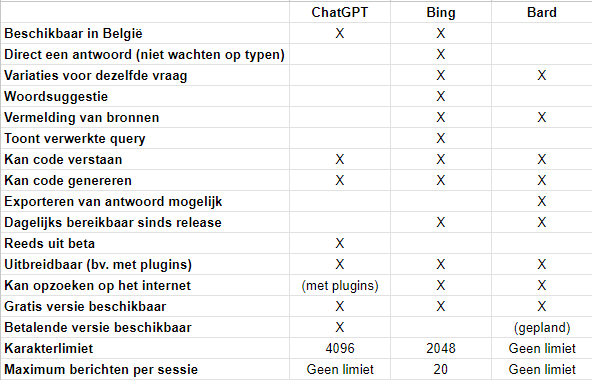
\includegraphics[width=\textwidth]{vergelijking_ai_tools_programmeren.png}
\end{figure}
\label{ai_tools_agents}\subsection{AI-tools met AI-Agents}
Volgende AI-tools maken gebruik van AI-Agents om (sub)taken uit te voeren. Deze tools kunnen naar de toekomst toe zeer relevant worden in de IT-sector om grotere of complexere taken uit te voeren, die voor voorgaande AI-tools op moment van schrijven nog niet haalbaar zijn (bv. haal op volgende webpagina alle artikelen op waarvan de prijzen tussen de €20 en €50 euro liggen, en steek alles in .csv bestand). Beide tools zijn reeds aan bod gekomen in het hoofdstuk \ref{eervolle_vermeldingen}.
\\\\
Op moment van schrijven zijn deze AI-tools steeds meer en meer van elkaars functionaliteiten aan het overnemen. Het is daarom niet uitsluitend dat op een gegeven moment deze tools allemaal hetzelfde kunnen. De grootste factor bij het kiezen van een tool is persoonlijke voorkeur op vlak van lay-out, die zeer verschillend is tussen deze tools.
\begin{itemize}
    \item Auto-GPT
    \item AgentGPT
    \item Godmode
\end{itemize}
\label{ai_tools_volledige_ontwikkeling}\subsection{AI-tools voor volledige ontwikkeling}
Afhankelijk van hoe volgende AI-tools evolueren kunnen deze een mogelijks grote impact spelen in de ontwikkeling en overname van een webshop. 
\begin{itemize}
    \item 10Web (exporteren van een afgewerkt product is helaas (nog) niet mogelijk)
    \item Elementor AI (reeds besproken in het hoofdstuk 'Eervolle vermeldingen' \ref{elementor_ai_hoofdstuk})
\end{itemize}    
\subsection{Criteria}
De bovenstaande AI-tools kunnen met elkaar vergeleken worden op basis van heel wat meetbare aspecten. Het is aan de gebruiker zelf om hierin een besluit te trekken op basis van prioriteiten, beschikbare budget enzovoort. Een aantal van deze aspecten zijn:
\begin{itemize}
    \item de prijs
    \begin{itemize}
        \item gratis
        \item betalend met een eenmalige kost
        \item betalend met abonnement (in verschillende types)
    \end{itemize} 
    \item de uitvoeringssnelheid
    \begin{itemize}
        \item traag
        \item normaal
        \item snel
        \item snel (tegen betaling)
    \end{itemize} 
    \item de export limieten
    \begin{itemize}
        \item exporteerbaar
        \item enkel gebruik binnen AI-tool
    \end{itemize}
    \item integratie met een CMS
    \begin{itemize}
        \item niet mogelijk
        \item mogelijk voor WordPress
        \item mogelijk maar niet voor WordPress
    \end{itemize}
    \item automatisch opvullen van data
    \begin{itemize}
        \item mogelijk
        \item niet mogelijk
    \end{itemize}
    \item ...    
\end{itemize}
Op moment van schrijven is er nog geen tool gevonden die het hele proces kan automatiseren. Daarnaast loopt men het risico dat een AI-tool ook niet beschikbaar kan zijn (bv. bij downtime van de server door grote overlast van gebruikers). Voornamelijk ChatGPT heeft hier last van. Het is daarom aangeraden om met zo veel mogelijk verschillende AI-tools te werken, en zelf te bepalen hoe men deze implementeert.
\subsection{De webshops van Team Made}
Team Made heeft volgende lijst van webshops meegegeven (zie hieronder). Op moment van schrijven staat Mr. Teddybeer niet op een WordPress-omgeving, maar zij wensen op termijn wel over te schakelen.
\begin{itemize}
    \item Coureur Local (https://www.coureurlocal.be/)
    \item A bloc (https://www.a-bloc.be/)
    \item Angar (https://angar.be/)
    \item Mr. Teddybeer (https://www.mr-teddybeer.be/)
    \item Wittevrongel (https://www.agrowittevrongel.be/)
    \item Petites Jubelles (https://petites-jubelles.be/)
    \item Kwiek en kwispel (https://kwiekenkwispel.be/)
    \item My shirt matters (https://myshirtmatters.com/)
    \item Motorcycle cushions (https://motorcyclecushions.net/)
\end{itemize} 
\subsection{Scenario's}
De mogelijke scenario's die kunnen optreden bij het overnemen van een webshop zijn als volgt:
\begin{itemize}
    \item Geen WordPress
    \begin{itemize}
        \item toegang tot MySQL databank
        \item geen toegang tot MySQL databank
        \item geen MySQL databank
        \begin{itemize}
           \item overzetten naar MySQL
           \item niet kunnen overzetten
       \end{itemize} 
    \end{itemize}
    \item Wel WordPress 
    \begin{itemize}
        \item toegang tot de site
        \begin{itemize}
            \item toegang tot de databank
            \begin{itemize}
                \item met WooCommerce export
                \item zonder WooCommerce export
            \end{itemize} 
            \item geen toegang tot de databank
            \begin{itemize}
                \item met WooCommerce plugin actief
                \item zonder WooCommerce plugin actief
            \end{itemize} 
        \end{itemize} 
        \item geen toegang tot de site
        \begin{itemize}
            \item met WooCommerce plugin actief
            \item zonder WooCommerce plugin actief
        \end{itemize} 
    \end{itemize} 
\end{itemize} 
\section{Uitleg installatie}
Het installeren van een WordPress instantie verloopt in een aantal stappen die geautomatiseerd kunnen worden. In volgende hoofdstukken worden deze stappen besproken voor de webshop Coureur Local. Aangezien Team Made met Windows werkt zullen alle scripts en terminal commands geschreven zijn in een Windows-besturingssysteem.
\\\\
Merk op dat er per functionaliteit een script voorzien is (bv. een script om enkel en alleen een lege databank aan te maken\ref{aanmaken_database_script}). Dit is bewust gedaan zodat de gebruiker van het toekomstige stappenplan (zie \ref{ch:stappenplan}) eenvoudig stappen kan overslaan (indien gewenst). Dit geeft ook het voordeel van sneller mogelijks optredende fouten op te sporen. 
\subsection{Folderstructuur}
In een WordPress installatie zijn verschillende folders aanwezig die elk hun eigen functionaliteit hebben. De belangrijkste hiervan zijn:
\begin{itemize}
    \item wp-admin - hierin komt alle code te staan die specifiek voor de administrator is zoals het dashboard
    \item wp-content - deze folder is een van de belangrijkste en zal hieronder verder besproken worden
    \item wp-includes - hier zitten de basis functionaliteiten om de CMS te doen werken
\end{itemize} 

\subsection{De wp-content}
Bij het opstellen van een nieuwe webshop zal deze folder de meeste aanpassen krijgen. De belangrijkste subfolders hier zijn:
\begin{itemize}
    \item plugins - elke plugin wordt in deze folder geïnstalleerd
    \item themes - hierin komen de standaard WordPress-themes alsook de eigen custom themes terecht
    \item uploads - hier zitten alle mediabestanden zoals afbeeldingen en video's die worden geüpload 
\end{itemize} 
\subsection{Databank en sitegegevens}
Command-line tools of scripts kunnen de downloadlink van WordPress ophalen, het zipbestand downloaden en automatisch uitpakken naar de juiste locatie. WordPress werkt op een MySQL-databank, de aanmaak hiervan kan ook worden geautomatiseerd met behulp van scripts. Tenslotte kunnen een aantal webshop-gegevens reeds voorzien worden zoals de website titel, beschrijving, tijdzone en taal. Een standaard gebruiker instellen kan via deze weg ook. Merk op dat er nog meer instellingen kunnen aangevuld worden zoals de adminEmail, permalinkStructure, uploadsPath, defaultCategory enzovoort. Wat men visueel in WordPress van instellingen kan aanpassen, moet in theorie ook enkel en alleen in code lukken.
\subsection{Eigen thema (custom theme)}
WordPress werkt met thema's om de lay-out en design van een website te bewaren. Standaard installeert en activeert WordPress een thema van hen. Een custom theme is een thema dat je volledig zelf in beheer hebt. Dit geeft het voordeel van een volledig uniek design te implementeren, maar vergt bijgevolg wel meer kennis. Er zijn verschillende opties voor Team Made:
\begin{itemize}
    \item WordPress thema - blijf met het standaard thema werken
    \item eigen custom theme - maak zelf een custom theme (per project) aan
    \item download een custom theme - haal een (betalende) custom theme van het internet af en bewerk die
\end{itemize}
Voor veiligheidsredenen is het aangeraden om altijd een standaard WordPress thema gedownload te hebben. Mocht er een fout optreden met een custom theme dan kan WordPress daarop terugvallen. Het zal mogelijks voor een andere lay-out zorgen, maar de website zal geen foutmelding geven en niet onbeschikbaar/offline zijn. 
\subsection{WP-CLI}
Om de veiligheid en toekomstige compatibiliteit van het script te verbeteren kan men best werken met de WP-CLI (WordPress Command Line Interface) tool. Het is veiliger omdat het gebruikmaakt van de ingebouwde WordPress-beveiliging om ervoor te zorgen dat de ingevoerde gegevens worden gevalideerd. Dit helpt potentiële beveiligingsproblemen zoals SQL-injecties te voorkomen. Doordat het gebruikmaakt van de officiële WordPress-cli-functionaliteit is het minder waarschijnlijk dat het wordt beïnvloed door toekomstige updates of wijzigingen in de WordPress-codebase, en het langer zal blijven werken met toekomstige versies van WordPress.
\\\\
\section{Installatie benodigdheden}
De WP-CLI maakt gebruik van wp option update commando's. Om wp option update te gebruiken in een script, moet je eerst zorgen dat WP-CLI is geïnstalleerd op je systeem en dat het beschikbaar is in het pad (PATH). Hiervoor is PHP 5.4.0 of hoger nodig. De versie (en de locatie) kan je controleren in de terminal met volgend(e) commando('s):\begin{minted}{bash}
php --version
# Voor de locatie op te halen: php --ini
\end{minted}
\begin{figure}
    \caption{'Ophalen van PHP informatie'}
    \label{ophalen_php_info}
    \centering
    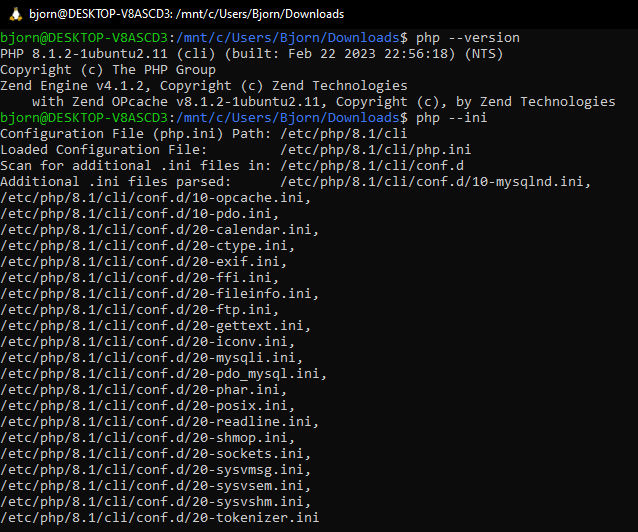
\includegraphics[width=\textwidth]{ophalen_php_info.png}
\end{figure}Zie figuur \ref{ophalen_php_info} voor een succesvol resultaat. Indien je geen antwoord krijgt dan moet je PHP nog installeren. Vervolgens moet je WP-CLI\footnote{\href{https://wp-cli.org/\#installing}{https://wp-cli.org/\#installing}} downloaden en installeren. Het is aangeraden om de officiële documentatie van WP-CLI te volgen, eventueel in combinatie met de documentatie op make.wordpress\footnote{\href{https://make.wordpress.org/cli/handbook/guides/installing/}{https://make.wordpress.org/cli/handbook/guides/installing/}}. 
\\\\
De stappen die moeten ondernomen worden op een Windows-besturingssysteem zijn als volgt:
\\\\
1. Haal de wp-cli.phar op met het commando:
\begin{minted}{bash}
# Kan ook met wget werken
curl -O https://raw.githubusercontent.com/wp-cli/builds/gh-pages/phar/wp-cli.phar
\end{minted}
2. Controleer in de folder of de .phar file werkt met het commando
\begin{minted}{bash}
php wp-cli.phar --info
\end{minted}
3. Vervolgens maak je het bestand uitvoerbaar met het commando
\begin{minted}{bash}
chmod +x wp-cli.phar
\end{minted}
4. Tenslotte verplaats je het bestand naar een globale plaats op de computer, een voorbeeld hiervan is
\begin{minted}{bash}
sudo mv wp-cli.phar /usr/local/bin/wp
\end{minted}
5. Een update voorzien kan met het commando
\begin{minted}{bash}
sudo wp cli update
\end{minted}
Dit zal bij een succesvolle installatie reageren met 'WP-CLI is at the latest version'. Tenslotte moet je het pad van wp-cli nog toevoegen aan de omgevingsvariable PATH op jouw systeem. Dit kan bij 'Edit the system environment variables > Advanced > Environment Variables > System variables > zoeken naar de variabele Path'. Pas hier de variabele aan.
\\\\
Je kan controleren of alles goed werkt door info op te halen via het commando:\begin{minted}{bash}
wp --info
\end{minted}
\begin{figure}
    \caption{'Ophalen van WP informatie'}
    \label{ophalen_wp_info}
    \centering
    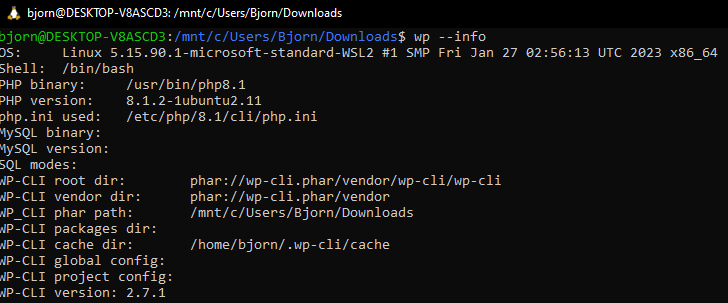
\includegraphics[width=\textwidth]{ophalen_wp_info.png}
\end{figure}Als alles goed is gelukt kan je voortaan globaal op de machine WP-CLI gebruiken. Zie figuur \ref{ophalen_wp_info} voor een voorbeeld van een succesvol resultaat. We kiezen voor dit globaal te gebruiken zodat alle (toekomstige) projecten dit kunnen hanteren (in plaats van per project een WP-CLI te downloaden). 
\\\\
Je kan op een Windows-besturingssysteem een script toevoegen door een tekstbestand toe te voegen, de lijnen code in te vullen en vervolgens de bestandsextensie te veranderen van .txt naar .sh. Om Shell-scripts te gebruiken op Windows heb je een Linux shell nodig en een command-language Bash. Je kan op Windows werken met deze scripts zonder Ubuntu te downloaden m.b.v. WSL (Windows Subsystem for Linux). Hiervoor ga je naar 'settings > update \& security > for developers >' en zet de knop 'Developer mode' aan. Vervolgens zoek je naar 'Turn Windows features on or off' en vink je de WSL map aan. Na de installatie kan een herstart van de computer noodzakelijk zijn. 
\\\\
Voor deze proof-of-concept zal op bepaalde plaatsen met WLS worden gewerkt. We werken met XAMPP Control Panel (v3.3.0), waarbij we de modules Apache en MySQL aanzetten, en de WordPress databank bijhouden in phpMyAdmin (MySQL/MariaDB). Merk op dat de namen van files en directories specifiek voor een computer geschreven zijn, en voor eigen toepassing mogelijks zullen verschillen. Het is daarom aangeraden om een voorbeeldscript eerst aandachtig door te nemen vooraleer men deze overneemt. De voorbeeldscripts maken gebruik van MySQL. Om te controleren of dit reeds geïnstalleerd is kan men volgend commando gebruiken:
\begin{minted}{bash}
mysql --version 
\end{minted}
Indien het nog niet geïnstalleerd is kan men dit doen met het commando:
\begin{minted}{bash}
sudo apt install mysql-client
\end{minted}
Voor het uitpakken van zip-bestanden (nodig voor de plugins) is 'unzip' nodig. Dit kan men installeren via het commando:
\begin{minted}{bash}
sudo apt-get install unzip
\end{minted}
Update: sinds het schrijven is deze plugin zeer onstabiel geworden. Een beter alternatief is 7zip die overigens ook een progressie toont bij het uitvoeren van een commando. Deze kan men installeren via het commando:
\begin{minted}{bash}
sudo apt install p7zip p7zip-full p7zip-rar
\end{minted}
\section{Uitvoeren van scripts}
Open Linux shell in de map waar het script in staat en typ het commando:\begin{minted}{bash} 
bash naamVanHetScript.sh
\end{minted}
Dit zal het script uitvoeren. Indien je een foutmelding krijgt zoals '... command not found' dan moet je mogelijks nog een EOL conversie uitvoeren naar Unix. Dit kan in het programma Notepad++ door het script te openen en vervolgens op Edit > EOL conversion > Unix (LF) te klikken. Dit kan ook m.b.v. een commando:
\begin{minted}{bash}
chmod +x naamVanHetScript.sh
\end{minted}
Om een visuele status van de WordPress download te tonen gebruiken we Pipe Viewer. Dit kan men installeren op Windows 10 met het commando:\begin{minted}{bash}
sudo apt-get install pv
\end{minted}
Dit is om de gebruiker een duidelijke indicatie te geven wanneer alle bestanden gedownload zijn. Wanneer het script start zal direct een WordPress folder worden aangemaakt, maar nog niet alle bestanden zullen gedownload zijn. Het is daarom aangeraden om te wachten tot het script volledig is uitgevoerd. 
\section{Voorbeeldscripts}
\label{klantgegevens_coureur_local}\subsection{Configuratiebestand}
Wachtwoorden en andere gevoelige gegevens worden best veilig opgeslagen in een aparte bestand en worden best niet zomaar weergegeven in een ander script. Het grote voordeel aan deze werkwijze is dat alle noodzakelijke gegevens voor de installatie op één centrale plaats komen te staan. Op de WordPress website\footnote{\href{https://wordpress.org/documentation/article/settings-general-screen/}{https://wordpress.org/documentation/article/settings-general-screen/}} kunnen alle mogelijke settings om aan te passen worden teruggevonden. Een uitgewerkt voorbeeld van zo een configuratiebestand in Bash voor de klant Coureur Local ziet er als volgt uit:
\begin{minted}[breakanywhere=true]{bash}
#!/bin/bash
# Configuratiebestand voor Coureur Local
# Naam = klantgegevens_coureur_local.sh

# Database-instellingen
dbName="wp_coureur_local"
dbUser="root"
dbPassword=""
dbHost="localhost"
dbPort="3306"
dbPrefix="wp_"

# Site-instellingen
siteTitle="Coureur Local"
siteDescription="Koop bij ons jouw nieuwe fiets."
siteTimezone="Europe/Amsterdam"
siteLanguage="nl_NL"
siteUrl="https://coureurlocal.be"

# Standaard gebruiker instellen
defaultUsername="Admin"
defaultPassword="admin_wachtwoord"
defaultEmail="admin@teammade.be"

# WordPress-map pad
wordpressPath="C:/Users/Bjorn/Desktop/local_repos/hogent/bachelorproef/coureur_local/wordpress"

# Thema instellingen
author="Team Made"
themesPath="/wordpress/wp-content/themes"
themeName="Thema Coureur Local"
themeDescription="Thema speciaal voor Coureur Local gemaakt."

# Exporteer variabelen voor gebruik in andere scripts
export dbName
export dbUser
export dbPassword
export dbHost
export dbPort
export dbPrefix
export siteTitle
export siteDescription
export siteTimezone
export siteLanguage
export siteUrl
export defaultUsername
export defaultPassword
export defaultEmail
export wordpressPath
export author
export themesPath
export themeName
export themeDescription
\end{minted}

\subsection{Downloaden van WordPress}
Een voorbeeldscript in Bash (en uitgevoerd in Linux shell) voor WordPress automatisch op te halen, installeren en de progressie te tonen:
\label{opzet_wp_script}\begin{minted}{bash}
#!/bin/bash
# Naam script = opzet_wp.sh

# Ophalen van configuratiebestand klantgegevens_coureur_local.sh
source klantgegevens_coureur_local.sh

# Downloaden en uitpakken van WordPress met Pipe Viewer
curl -# -L "https://wordpress.org/latest.tar.gz" | pv -p -t -e -b -a | tar -xzf - >/dev/null

echo "WordPress is geïnstalleerd."
\end{minted}
Dit zal een volledig nieuwe WordPress-folder aanmaken met een standaard wp-config-sample.php in. Vervolgens gaan wij een eigen wp-config.php laten genereren met de juiste databankgegevens (die opgesteld zijn in 'klantgegevens\_coureur\_local.sh'\ref{klantgegevens_coureur_local}) met een nieuw script.

\subsection{Wp-config genereren en aanpassen}
Voor het aanmaken van de wp-config-file (op basis van de sample file), de databasegegevens in te vullen en een standaard gebruikersaccount aan te maken (die ook reeds opgesteld zijn in 'klantgegevens\_coureur\_local.sh') kunnen we volgend script gebruiken:
\label{aanpassen_config_script}\begin{minted}{bash}
#!/bin/bash
# Naam script = aanpassen_wp_config.sh

# Ophalen van configuratiebestand klantgegevens_coureur_local.sh
source klantgegevens_coureur_local.sh

# WordPress Configuratiebestand aanmaken
cp "wordpress/wp-config-sample.php" "wordpress/wp-config.php"

# Check of het configuratiebestand is aangemaakt
if [ -f "wordpress/wp-config.php" ]; then
echo "Configuratiebestand is aangemaakt: $wordpressPath/wp-config.php"
else
echo "Fout bij het aanmaken van het configuratiebestand."
exit 1
fi

# Associative array met databasegegevens en WordPress-site instellingen
declare -A replacements=(
['DB_HOST']="$dbHost"
['DB_PORT']="$dbPort"
['DB_USER']="$dbUser"
['DB_PASSWORD']="$dbPassword"
['DB_NAME']="$dbName"
['WP_HOME']="$siteUrl"
['WP_SITEURL']="$siteUrl"
['WP_TITLE']="$siteTitle"
['WP_DESCRIPTION']="$siteDescription"
['WP_TIMEZONE']="$siteTimezone"
['WP_LANG']="$siteLanguage"
)

# Functie om databasegegevens te vervangen in het configuratiebestand
function replace_database_value() {
    local key="$1"
    local value="$2"
    perl -i -pe "s|define\(\s*'$key',\s*\K.*?(?=\);)|'$value'|g" "wordpress/wp-config.php"
}

# Vervangen van databasegegevens en WordPress-site instellingen in het configuratiebestand
for key in "${!replacements[@]}"; do
replace_database_value "$key" "${replacements[$key]}"
done

echo "WordPress databasegegevens zijn automatisch ingevuld en een standaard gebruikersaccount is aangemaakt."
\end{minted}
Hierin worden alle variabelen aangepast in de nieuwe wp-config.php met de eerder opgegeven klantgegevens. De sample-file kan blijven staan als eventuele back-up. Zodra er een eigen wp-config.php aanwezig is zal de sample niet langer aangesproken worden.
\\\\
We kunnen vanaf volgende stappen de automatisch gegenereerde WordPress-folder verplaatsen naar de 'htdocs' folder van XAMPP. Als we navigeren in een browser naar http://localhost/wordpress/ dan komen we op een WordPress installatie uit. De phpMyAdmin kunnen we bereiken via http://localhost/phpmyadmin. Hierbij kijkt de installatie naar de aanwezige wp-config om een connectie te maken met de databank. Op dit ogenblik is er echter nog geen databank aanwezig en zal de installatie dus falen. Merk op dat de opgegeven urls mogelijks kunnen verschillen van systeem.
\\\\
\label{aanmaken_database_script}\subsection{Databank opstellen}
Het aanmaken van een databank en gebruiker in phpMyAdmin kan manueel door volgende stappen te ondernemen:
\begin{itemize}
    \item Onder het tabblad 'Databases' geef je een naam op en maak je een database aan met als type utf8mb4\_general\_ci
    \item Vervolgens voeg je onder het tabblad 'Users' een gebruiker toe
    \item Bewerk indien gewenst de rechten van de gebruiker door helemaal rechts in het overzicht op 'Edit privileges' te klikken
\end{itemize}
Eens dat deze stappen zijn voltooid is een databank klaar om gekoppeld te worden. Wanneer alle data van WordPress is voorzien (na de installatie) kan de tabel worden geoptimaliseerd in het tabeloverzicht van phpMyAdmin.
\\\\
Het grote nadeel aan deze stap te willen automatiseren is dat de databank enkel zal werken in een lokale omgeving. Dit komt omdat de data in de tabel wp\_options bij de 'siteurl' en 'home' op een lokale url staan (zie afbeelding \ref{wp_options_phpmyadmin}). 
\begin{figure}
    \caption{'De wp options in phpMyAdmin'}
    \label{wp_options_phpmyadmin}
    \centering
    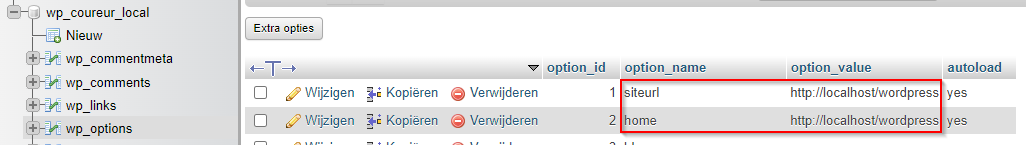
\includegraphics[width=\textwidth]{wp_options_phpmyadmin.png}
\end{figure}Het is aangeraden om voor de ontwikkeling van een databank voorkeur te geven aan een databank die reeds live staat. Afhankelijk van de hosting die Team Made gebruikt kan zo een live databank op dezelfde wijze als een lokale databank (sneller) aangemaakt worden. Dit geeft het grote voordeel dat een lokale databank niet meer geëxporteerd en geïmporteerd moet worden naar een live databank. Men kan direct op een lokale omgeving met reële data werken.
\\\\
Indien men toch met een lokale databank wilt werken is het aangeraden om deze manueel uit te voeren (via phpMyAdmin) i.p.v. met scripting. Het huidige installatieproces van WordPress is zeer snel. In theorie kan alles m.b.v. de WP-CLI in scripting worden weggeschreven. Een voorbeeld hiervan is:
\begin{minted}{bash}
#!/bin/bash
# Naam script = aanmaken_database_wp.sh

# Get klantgegevens_coureur_local.sh
source klantgegevens_coureur_local.sh

wp db create --dbuser="$dbUser" --dbpass="$dbPassword"
\end{minted}
In het script 'aanmaken\_database\_wp.sh' halen we opnieuw de geëxporteerde variabelen van de 'klantgegevens\_coureur\_local.sh' op. Merk op dat paramaters zoals de dbName niet mogelijk zijn in het wp db create commando. Deze gaat zelf op basis van uw wp-config-file beslissen hoe de databank zal noemen. Ook zal de databank van de collation 'utf8mb4\_0900\_ai\_ci' zijn i.p.v. 'utf8mb4\_general\_ci'. Om dit op te lossen kan je inloggen op de MySQL/MariaDB server, en vervolgens de databank te wijzigen met het commando:
\begin{minted}{bash}
ALTER DATABASE wp_coureur_local COLLATE = utf8mb4_general_ci;
\end{minted}
Opgelet: indien je meerdere mysql instanties heb geïnstalleerd op de computer, zal de databank worden aangemaakt in één van deze data folders op basis van de eerder ingevulde systeemvariabele PATH. Ook zal de databank nog niet verschijnen omdat deze nog leeg is. Indien je een lege databank rechtstreeks zou aanmaken in phpMyAdmin dan gaat deze wel direct in de lijst verschijnen.
\label{eigen_thema_script}\subsection{Eigen thema opzetten}
Indien er gekozen wordt om een volledig nieuw custom theme aan te maken en te activeren, kan dit ook met behulp van scriptie.
Een voorbeeld van een Bash script voor het aanmaken en activeren van een eigen thema (custom theme) dat opnieuw gebruikmaakt van de klantengegevens:
\begin{minted}{bash}
#!/bin/bash
# Naam script = eigen_thema_wp.sh

# Ophalen van configuratiebestand klantgegevens_coureur_local.sh
source klantgegevens_coureur_local.sh

# Navigate to the themes directory
cd "wordpress/wp-content/themes/"

# Create the custom theme folder
mkdir -p "$themeName"

# Navigate back to root
cd "../../../"

currentDirectory=$(pwd)

# Add a theme image to the theme folder
sampleImage="$currentDirectory/../assets/coureurlocalrond150.png"
destinationImagePath="$currentDirectory/$themesPath/$themeName/styles.png"
cp "$sampleImage" "$destinationImagePath"

# Create the necessary theme files
styleFilePath="$currentDirectory/$themesPath/$themeName/style.css"
indexFilePath="$currentDirectory/$themesPath/$themeName/index.php"

# Generate the content for the style.css file
styleContent="/*
Theme Name: $themeName
Description: $themeDescription
Version: 1.0
Author: $author
*/

/* Additional CSS styles go here */"
echo "$styleContent" > "$styleFilePath"

# Generate the content for the index.php file
indexContent="<?php
// Silence is golden.
"
echo "$indexContent" > "$indexFilePath"

# Download wp-cli if it doesn't exist
if [ ! -f "wordpress/wp-cli.phar" ]; then
    echo "Downloading wp-cli..."
    curl -O https://raw.githubusercontent.com/wp-cli/builds/gh-pages/phar/wp-cli.phar
    chmod +x wp-cli.phar
    mv wp-cli.phar wordpress/
fi

# Activate the custom theme
command="./wordpress/wp-cli.phar --path='./wordpress' theme activate '$themeName'"
eval "$command"

# Output success message
echo "Custom theme '$themeName' is geïnstalleerd en geactiveerd."
\end{minted}
Via deze weg kan heel eenvoudig per klant een custom theme worden aangemaakt door enkel het configuratiebestand ('klantgegevens\_coureur\_local.sh' in dit geval) manueel in te vullen, en een afbeelding te voorzien op dezelfde plaats als aangegeven in dat bestand.

\subsection{WooCommerce plugin downloaden}
Eens een WordPress installatie volledig opgezet is dan kan een admin zich inloggen en visueel plugins beheren. Het is echter ook mogelijk om via scriptie een plugin te downloaden en vervolgens te installeren in de WordPress-installatie. Deze nieuwe plugin komt dan ook terecht in de directory /wp-content/plugins. Ook dit bespaart manueel werk als op voorhand reeds geweten is welke plugin(s) zullen worden gebruikt.
\\\\
Belangrijk om in het achterhoofd te houden is dat plugins geschreven zijn door mensen die (meestal) niet per se van WordPress zelf zijn. Hou er rekening mee dat plugins beveiligingsrisico's met zich meenemen en mogelijks uw webshop kwetsbaar kunnen maken zoals Advanced Custom Fields (Pro) die in oudere versies XSS-aanvallen toelaat \autocite{Leemputten2023}. Het is aan de programmeur om te bepalen welke versie je neemt van de plugin, en of je de plugins automatisch laat updaten door WordPress of niet. Een mogelijke reden om niet automatisch te willen updaten kan het breken van compatibiliteit met andere plugins of andere WordPress functionaliteiten zijn.
\\\\
Een voorbeeldscript voor het downloaden van de WooCommerce plugin (activeren in de plugins folder):
\label{install_woocommerce_script}\begin{minted}{bash}
#!/bin/bash
# Naam script = install_woocommerce.sh

# Set the plugins path
pluginsPath="$PWD"

# WooCommerce plugin download URL
woocommerceUrl="https://downloads.wordpress.org/plugin/woocommerce.latest-stable.zip"

# WooCommerce plugin name and downloaded ZIP file name
woocommerceName="woocommerce" 
woocommerceFileName="$woocommerceName.zip"

# Download WooCommerce plugin
woocommerceFilePath="$PWD/$woocommerceFileName"
wget "$woocommerceUrl" -O "$woocommerceFilePath"

# Extract WooCommerce plugin to the plugins folder
7z x "$woocommerceFilePath" -o"$pluginsPath"

# Delete the zipped download file
rm "$woocommerceFilePath"

# Display success message
echo "WooCommerce plugin is downloaded, unzipped, and the zipped download is deleted."
\end{minted}
Dit script zal enige tijd in beslag nemen: de bestandsgrootte kan variëren van de versie maar zit op moment van schrijven rond de 10 MB. Merk op dat de plugin hiermee niet geactiveerd is. Dit kan met volgende uitbreiding in hetzelfde script (zie \ref{install_woocommerce_script}):
\begin{minted}{bash}
# WordPress Plugin API activation
apiPath="$wordpressPath/wp-load.php"
source "$apiPath"

# Activate WooCommerce plugin using Plugin API
pluginPath="$pluginsPath/$woocommerceName"
wp plugin activate "$woocommerceName"    
\end{minted}
Het is aangeraden om de activatie van de plugin manueel te doen in het adminpaneel van WordPress om een beter overzicht te behouden. Indien gewenst is het mogelijk om de automatische updates van WordPress direct aan te zetten door hetzelfde script (zie \ref{install_woocommerce_script}) uit te breiden met:
\begin{minted}{bash}
command="$wordpressPath/wp-cli.phar --path=$wordpressPath plugin update-all --allow-root"
eval "$command"
\end{minted}
Ook voor dit voorbeeldscript maken we gebruik van het configuratiebestand 'klantgegevens\_coureur\_local.sh'. Natuurlijk kan ook gekozen worden om het plugin pad hierin te steken. Plugins kunnen ook een activeerscript hebben, maar de paden hiervan kunnen variëren van plugin tot plugin. Dit probleem los je op door met de WordPress Plugin API te werken. Merk op dat het commando 'Active-Plugin' de WordPress Plugin API nodig heeft, die in de wp-load.php zit. Afhankelijk van Team Made hun voorkeuren kan men ervoor kiezen om:
\begin{itemize}
    \item per plugin een script te schrijven, en die één voor één te laten uitvoeren
    \item een combinatie van (veelgebruikte) plugins in één script te steken, om per project eenmalig uit te voeren
    \item alle scripts tot één script te combineren
\end{itemize} 
Het is aangewezen te wachten met het installeren van plugins in verband met beveiliging totdat de webshop live staat. Dit omdat deze plugins (bv. Wordfence) een firewall installeren, die bij het deployen van een webshop dubbel werk kunnen geven.
\section{Styling van lay-out}
Indien er voor een custom theme wordt gekozen en de styling volledig vanaf nul moet worden overgenomen, zijn er op moment van schrijven weinig AI-tools om daarbij te helpen. Het grote probleem is dat afbeelding-herkenningen nog niet aanwezig zijn in de publiek toegankelijk AI-tools. Deze zouden echter de beste oplossing zijn voor dit probleem. Naar toekomstig gebruik toe kan een gebruiker op basis van een screenshot vragen om het in code om te zetten. Op moment van schrijven moet de gebruiker zelf zeer duidelijk specifiëren wat hij wilt, wat zeer omslachtig is. Daarom is het sterk aangeraden om voor deze stap nog met een front-end developer te werken.
\section{Overname van data}
Voor het ophalen van goederen en/of diensten hun data zijn er verschillende opties aanwezig. Voor de auteur was het op moment van schrijven niet mogelijk om op de bèta versie alle functionaliteiten van AgentGPT te testen, maar webscraping bleek wel (in beperkte mate) goed te werken. Indien dit in de toekomst blijft werken (of zal verbeteren) is dit een zeer gebruiksvriendelijke werkwijze om zonder extra tools data van een webpagina op te halen. Merk op dat AgentGPT gebruikmaakt van een Python bibliotheek Beautiful Soup\footnote{\href{https://www.crummy.com/software/BeautifulSoup/bs4/doc/}{https://www.crummy.com/software/BeautifulSoup/bs4/doc/}} om data op te halen van een webpagina (zie figuur 3.1). 
\begin{figure}
    \caption{'AgentGPT gebruikt BeautifulSoup voor het ophalen van data op een webpagina'}
    \begin{center}
        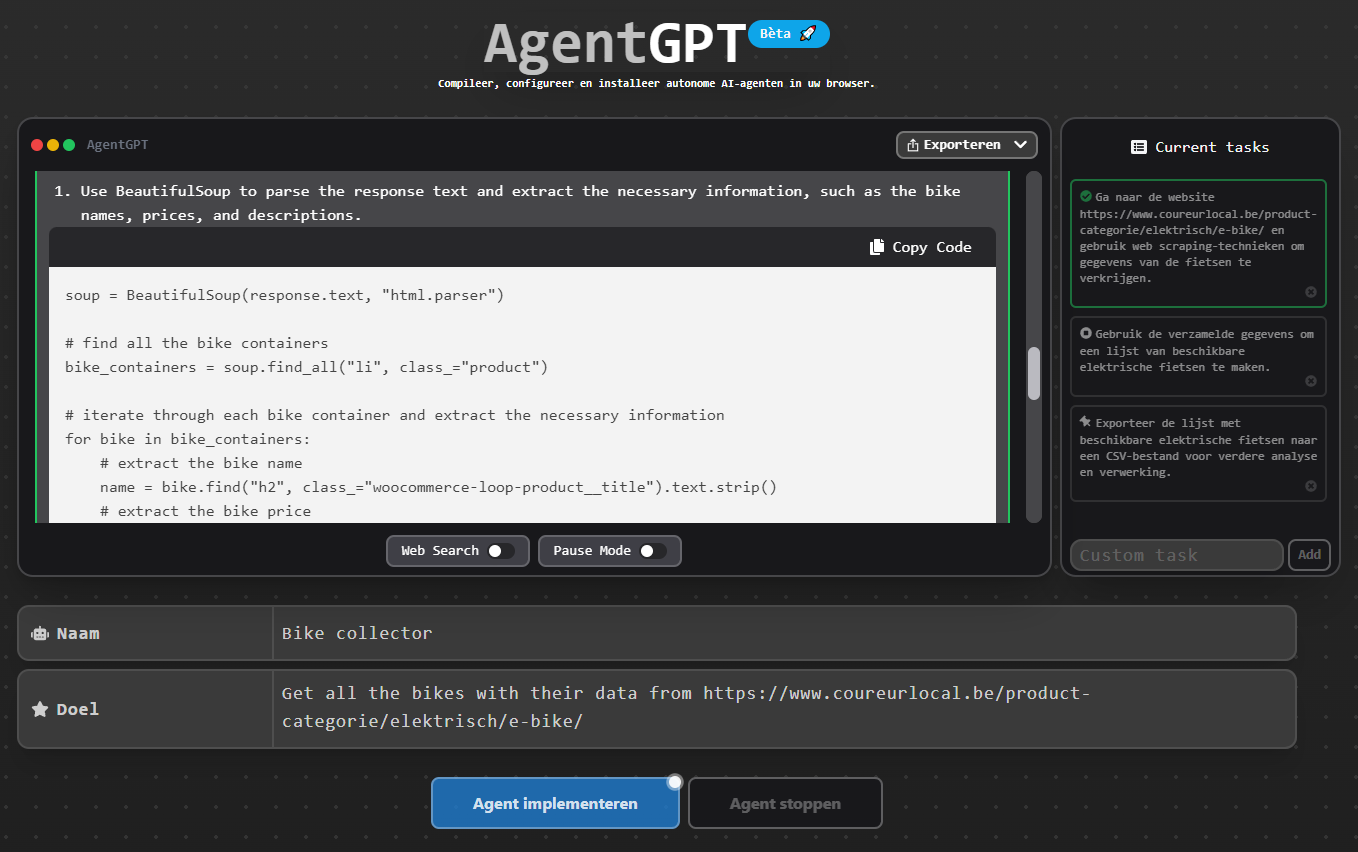
\includegraphics[width=\textwidth, height=\textheight, keepaspectratio]{agentgpt_uses_beautifulSoup}
    \end{center}
\end{figure} 
\\\\
ChatGPT kan op moment van schrijven al bestaande data omzetten naar nieuwe type data. Hiermee kan je een .csv-file aanmaken met de verkregen data, mocht die nog niet in een .csv-file zitten, om vervolgens te importeren met in de WooCommerce plugin\footnote{\href{https://woocommerce.com/document/importing-woocommerce-sample-data/}{https://woocommerce.com/document/importing-woocommerce-sample-data/}}.
\\\\
Voor data te importeren in WooCommerce heb je een CSV- of XML-bestand nodig. Vervolgens moet je meegeven welke velden van het bestand overeenstemmen met de velden van WooCommerce. Enkel een administrator met genoeg rechten op WordPress kan de importeer-functionaliteit van deze plugin gebruiken.